%%%%%%%%%%%%%%%%%%%%%%%%%%% asme2e.tex %%%%%%%%%%%%%%%%%%%%%%%%%%%%%%%
% Template for producing ASME-format articles using LaTeX            %
% Written by   Harry H. Cheng                                        %
%              Integration Engineering Laboratory                    %
%              Department of Mechanical and Aeronautical Engineering %
%              University of California                              %
%              Davis, CA 95616                                       %
%              Tel: (530) 752-5020 (office)                          %
%                   (530) 752-1028 (lab)                             %
%              Fax: (530) 752-4158                                   %
%              Email: hhcheng@ucdavis.edu                            %
%              WWW:   http://iel.ucdavis.edu/people/cheng.html       %
%              May 7, 1994                                           %
% Modified: February 16, 2001 by Harry H. Cheng                      %
% Modified: January  01, 2003 by Geoffrey R. Shiflett                %
% Use at your own risk, send complaints to /dev/null                 %
%%%%%%%%%%%%%%%%%%%%%%%%%%%%%%%%%%%%%%%%%%%%%%%%%%%%%%%%%%%%%%%%%%%%%%

%%% use twocolumn and 10pt options with the asme2e format
\documentclass[cleanfoot,cleanhead,onecolumn,12pt,notitlepage]{asme2e}
\special{papersize=8.5in,11in}

\usepackage{listings}
\usepackage{graphicx}
\usepackage{amsmath}
\usepackage[hidelinks]{hyperref}
\lstset{
    breaklines=true, % break lines for files
    basicstyle=\scriptsize,
    numbers=left,
    showstringspaces=false,
    frame=l
}

%% The class has several options
%  onecolumn/twocolumn - format for one or two columns per page
%  10pt/11pt/12pt - use 10, 11, or 12 point font
%  oneside/twoside - format for oneside/twosided printing
%  final/draft - format for final/draft copy
%  cleanfoot - take out copyright info in footer leave page number
%  cleanhead - take out the conference banner on the title page
%  titlepage/notitlepage - put in titlepage or leave out titlepage
%  
%% The default is oneside, onecolumn, 10pt, final

%%% You need to remove 'DRAFT: ' in the title for the final submitted version.
\title{Computer Project \#3}

%%% first author
\author{Shaun Harris
    \affiliation{
	Department of Mechanical and Aerospace Engineering\\
	Utah State University \\
    Email: shaun.r.harris@gmail.com
    }
}


\begin{document}

\maketitle 



%%%%%%%%%%%%%%%%%%%%%%%%%%%%%%%%%%%%%%%%%%%%%%%%%%%%%%%%%%%%%%%%%%%%%%

\begin{abstract}
    {\it A staggard grid Navier-Stokes solver is implemented to solve a driven cavity problem, and a channel flow problem.  The Pressure, u-velocity and v-velocity are all staggard and solved for separatley.  The necessary equations and the implemented code is provided in this paper.}
\end{abstract}

%%%%%%%%%%%%%%%%%%%%%%%%%%%%%%%%%%%%%%%%%%%%%%%%%%%%%%%%%%%%%%%%%%%%%%

\begin{nomenclature}
\entry{$u$}{Velocity in the x-direction (m/s)}
\entry{$u_i$}{Velocity in the x-direction referencing neighbor $i (N,E,S,W,P)$ lowercase $(n,e,s,w)$ indicates averaged values}
\entry{$u_P^{old}$}{Velocity in the x-direction from previous iteration on node center}
\entry{$v$}{Velocity in the y-direction}
\entry{$v_i$}{Velocity in the y-direction referencing neighbor $i (N,E,S,W,P)$ lowercase $(n,e,s,w)$ indicates averaged values}
\entry{$v_P^{old}$}{Velocity in the y-direction from previous iteration on node center}
\entry{$P$}{Pressure}
\entry{$i'$}{Correction term for $i (u,v,P)$}
\entry{$a_{i,j}$}{Coefficient for final discretized equation referencing neighbor $i (N,E,S,W,P)$ on $j (u,v,P)$ mesh}
\entry{$\tilde{a}_{P,j}$}{Coefficient for final discretized equation referencing center $P$ on $j (u,v,P)$ mesh and divided by $\Omega$ correction factor}
\entry{$\Omega$}{non-linear correction factor for momentum equations}
\entry{$\Omega_P$}{linear correction factor for pressure equation}
\entry{$\alpha$}{Pressure blending factor}
\end{nomenclature}

%%%%%%%%%%%%%%%%%%%%%%%%%%%%%%%%%%%%%%%%%%%%%%%%%%%%%%%%%%%%%%%%%%%%%%
\clearpage

\tableofcontents   

\clearpage

\section{INTRODUCTION}

In order to solve the Navier Stokes equation in two dimensions a staggered grid approach was used.  This where the $u,v,$ and $P$ values were all saved in separate locations on the grid.  This allowed for many of the oscillations to be minimized and for the solution to converge to a correct solution.

Two cases were considered in this problem.  These cases were a driven cavity and a channel flow.  The inputs and requirements are shown on the problem outline.  

The numerical method, application with code, and results are shown in the following sections.


%%%%%%%%%%%%%%%%%%%%%%%%%%%%%%%%%%%%%%%%%%%%%%%%%%%%%%%%%%%%%%%%%%%%%%

\section{NUMERICAL METHOD}
In order to solve using this method, a staggered grid was utilized.  Fig. \ref{fig:stencil} shows how the $u,v,$ and $P$ values were saved on the grid.  The momentum equation is discretized from Eq. \ref{eq:umom} to \ref{eq:disumom}.  

\begin{figure}[h]
\begin{center}
    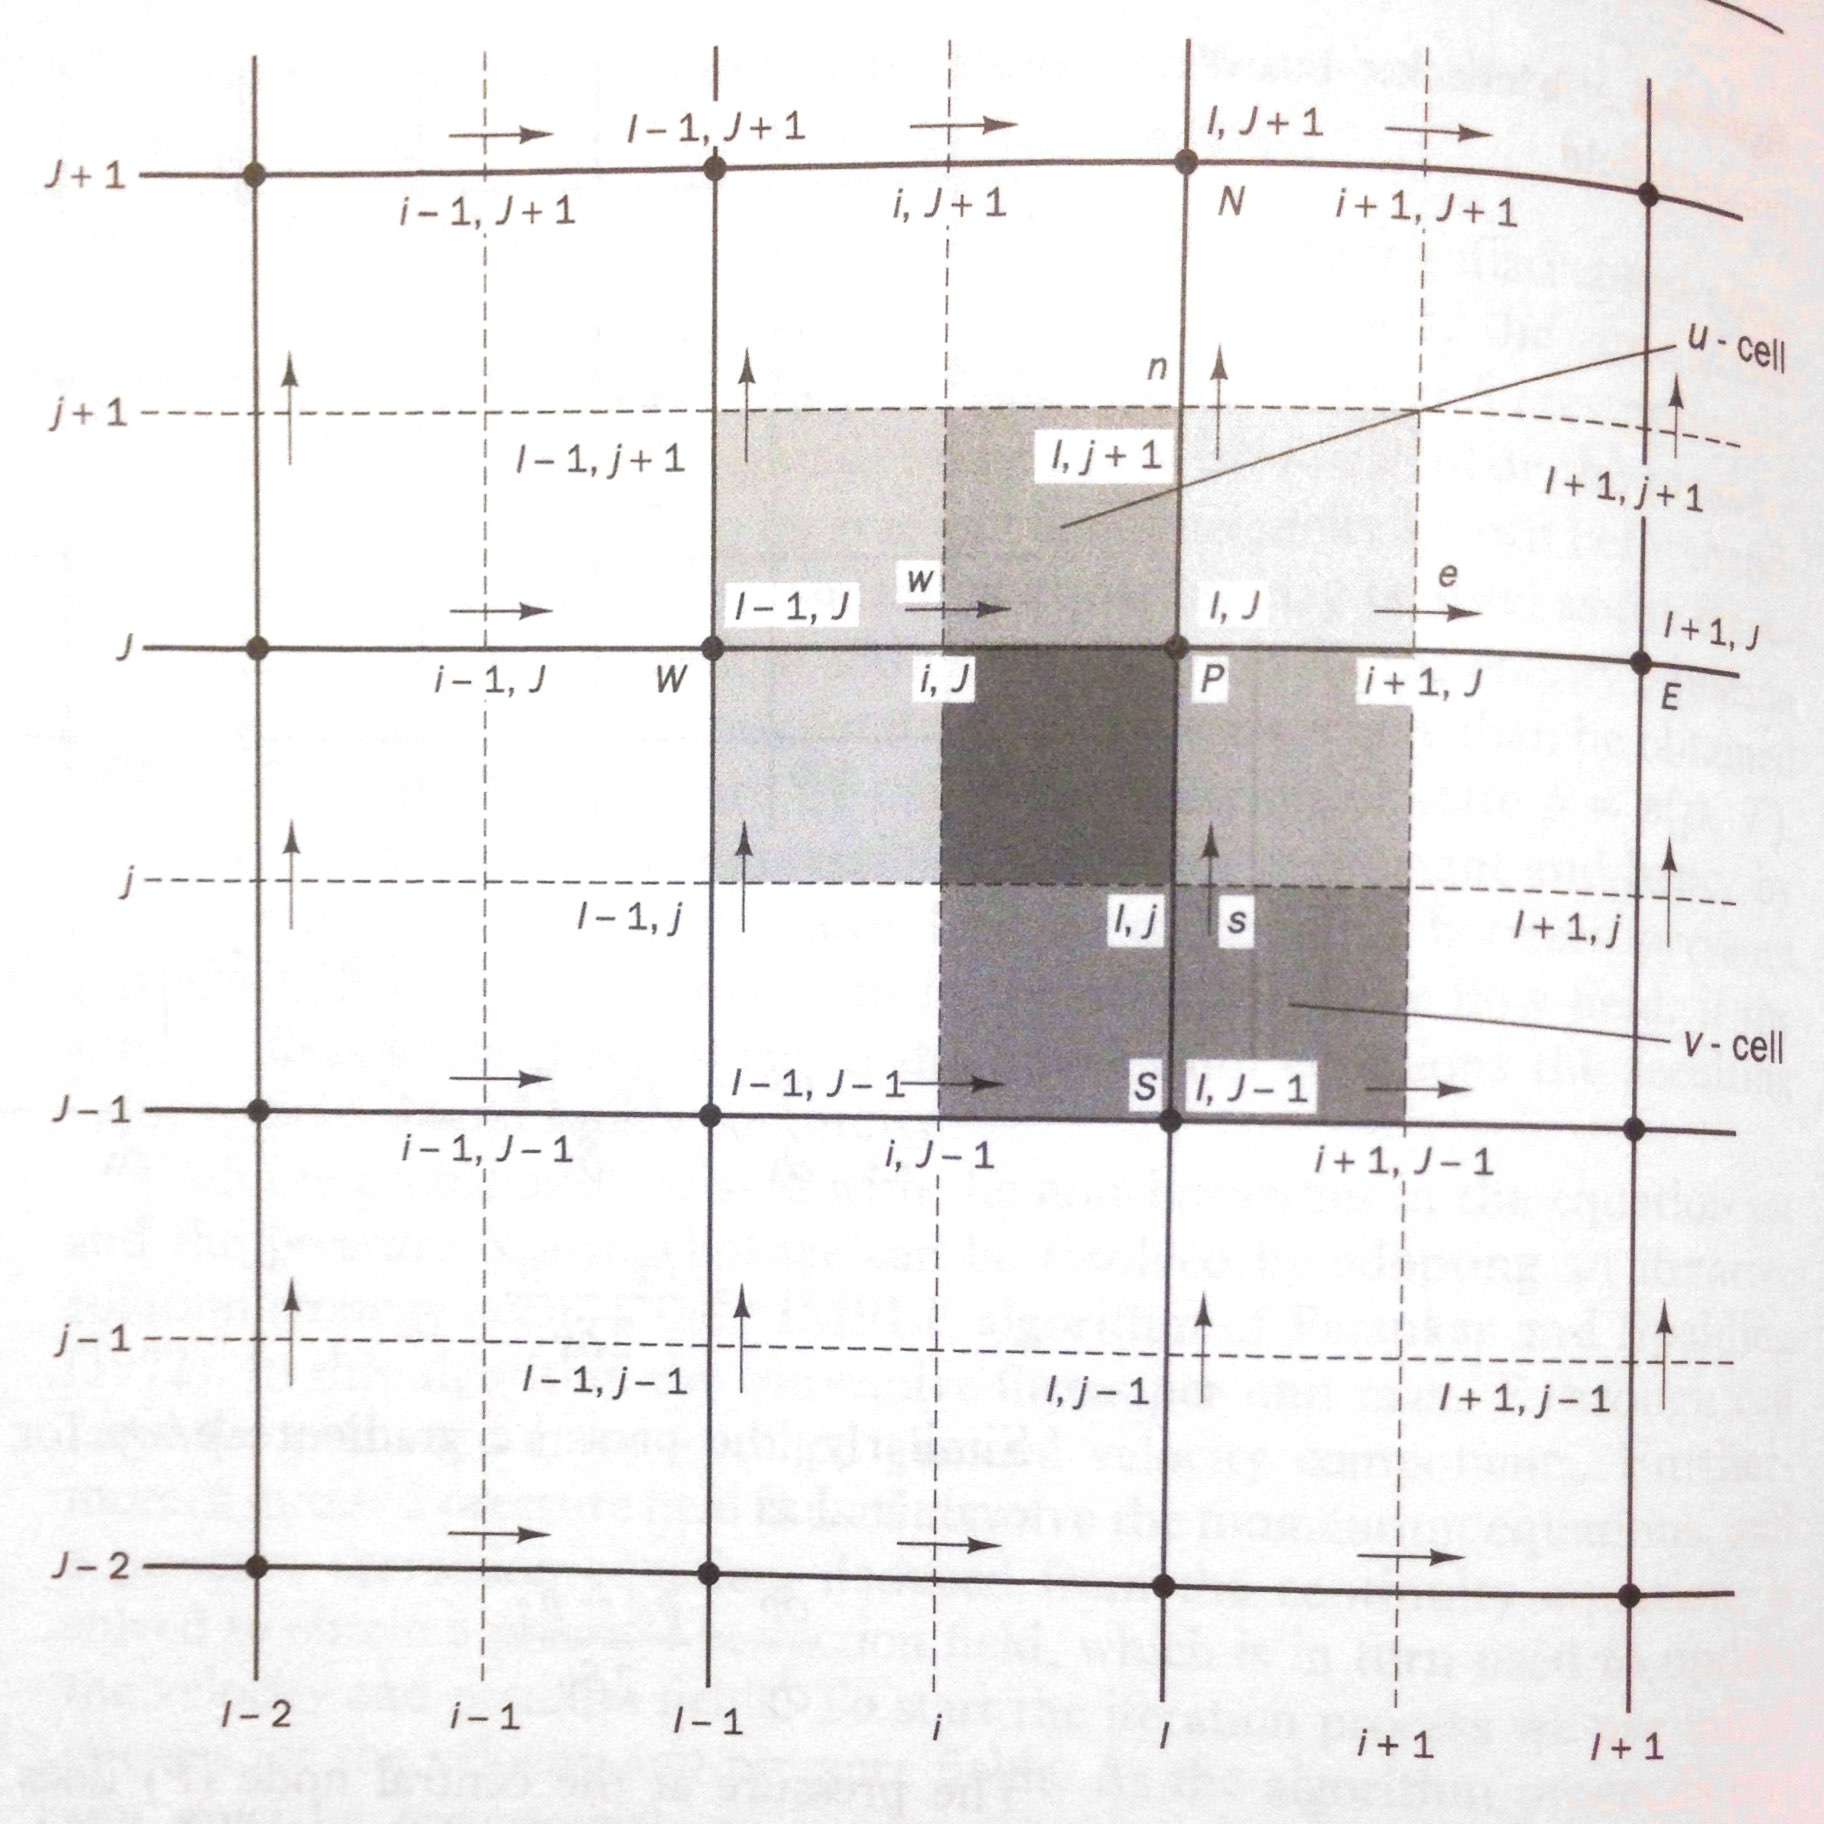
\includegraphics[width=0.9\linewidth]{Stencil.jpg}
    \caption{REPRESENTATION OF STENCIL FOR GRID GENERATION}
    \label{fig:stencil}
\end{center}
\end{figure}

\begin{equation}
\begin{aligned}
\frac{\partial (\rho u u)}{\partial x} + \frac{\partial (\rho v u)}{\partial y} &=
-\frac{\partial P}{\partial x} 
+ \frac{\partial }{\partial x} \left( \mu \frac{\partial u}{\partial x} \right)
+ \frac{\partial }{\partial y} \left( \mu \frac{\partial u}{\partial y} \right)
+ \frac{\partial }{\partial x} \left( \mu \frac{\partial u}{\partial x} \right)
+ \frac{\partial }{\partial y} \left( \mu \frac{\partial v}{\partial y} \right)
\label{eq:umom}
\end{aligned}
\end{equation}

\begin{equation}
\begin{aligned}
u_P &= (1 - \Omega) u_P^{old} + \frac{1}{\tilde{a}_{P,u}} 
	\left[a_{E,u} u_E
		+ a_{W,u} u_W
		+ a_{N,u} u_N
		+ a_{S,u} u_S
		+ dy (P_w - P_e)
	\right] \\
	\textit{where:} \\
	a_{E,u} &= max(-\rho u_e dy,0) + \mu dy / dx \\
	a_{N,u} &= max(-\rho v_n dx,0) + \mu dx / dy \\
	a_{W,u} &= max( \rho u_w dy,0) + \mu dy / dx \\
	a_{S,u} &= max( \rho v_s dx,0) + \mu dx / dy \\
\label{eq:disumom}
\end{aligned}
\end{equation}

The following equations (Eq. \ref{eq:vmom} and \ref{eq:disvmom}) show the discretized equations used for $v$ velocity momentum.  

\begin{equation}
\begin{aligned}
\frac{\partial (\rho u v)}{\partial x} + \frac{\partial (\rho v v)}{\partial y} &=
-\frac{\partial P}{\partial x} 
+ \frac{\partial }{\partial x} \left( \mu \frac{\partial v}{\partial x} \right)
+ \frac{\partial }{\partial y} \left( \mu \frac{\partial v}{\partial y} \right)
+ \frac{\partial }{\partial x} \left( \mu \frac{\partial u}{\partial x} \right)
+ \frac{\partial }{\partial y} \left( \mu \frac{\partial v}{\partial y} \right)
\label{eq:vmom}
\end{aligned}
\end{equation}

\begin{equation}
\begin{aligned}
v_P &= (1 - \Omega) v_P^{old} + \frac{1}{\tilde{a}_{P,v}} 
	\left[a_{E,v} v_E
		+ a_{W,v} v_W
		+ a_{N,v} v_N
		+ a_{S,v} v_S
		+ dy (P_s - P_n)
	\right] \\
	\textit{where:} \\
	a_{E,v} &= max(-\rho u_e dy,0) + \mu dy / dx \\
	a_{N,v} &= max(-\rho v_n dx,0) + \mu dx / dy \\
	a_{W,v} &= max( \rho u_w dy,0) + \mu dy / dx \\
	a_{S,v} &= max( \rho v_s dx,0) + \mu dx / dy \\
\label{eq:disvmom}
\end{aligned}
\end{equation}

It should be noted that these equations took into account the spacing on the boundary.  That is, if there was a ghost node that was used in the coefficient calculations, then the $\mu dx/dy$ like terms became $\mu 2 dx / dy$ terms on the North and South boundaries for the $u$ momentum calculations.  

The pressure was discretized from continuity, staggered control volume equations, and velocity correction terms.   Thus, the continuity equation shown in Eq. \ref{eq:p} is discretized to Eq. \ref{eq:disp}.  

\begin{equation}
\begin{aligned}
\frac{\partial (\rho u)}{\partial x}
+
\frac{\partial (\rho v)}{\partial y} 
&= 0
\label{eq:p}
\end{aligned}
\end{equation}

\begin{equation}
\begin{aligned}
P_P' &= P_P' + \frac{\Omega_P}{a_{P,P}}
\left(a_{E,P} P_E'
	+ a_{W,P} P_W'
	+ a_{N,P} P_N'
	+ a_{S,P} P_S'
	- S
	- a_{P,P} P_P'
\right)\\
P &= P^{old} + \alpha P'
\label{eq:disp}
\end{aligned}
\end{equation}

It should be noted that momentum is non-linear so the relaxation factors used were $\Omega \approx 0.6$ and the $\Omega_P \approx 1.7$ while $\alpha \approx 0.3$ for the linear pressure equation.


\begin{figure}[h!]
\begin{center}
    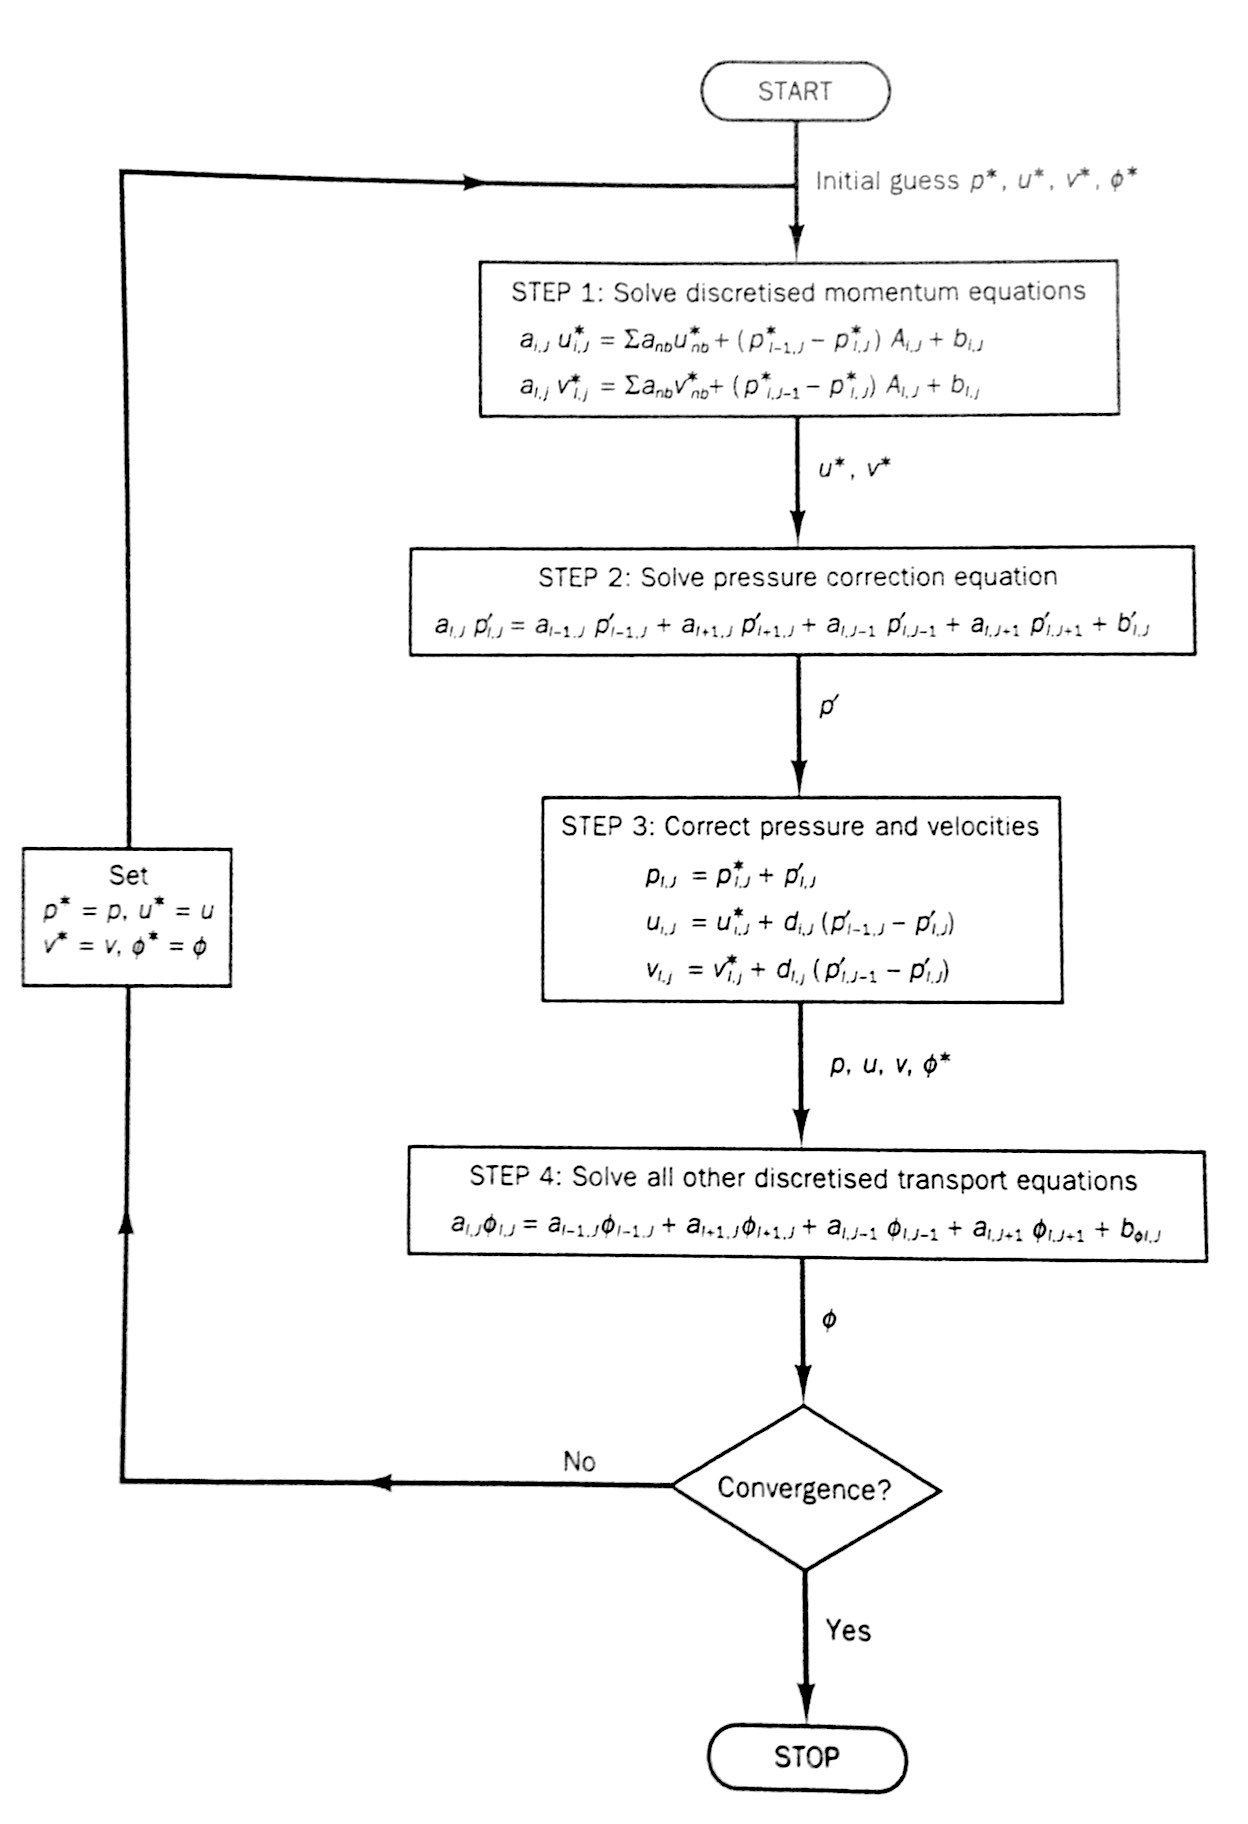
\includegraphics[width=0.7\linewidth]{Code_Outline.jpg}
    \caption{Outline of code structure}
    \label{fig:codeoutline}
\end{center}
\end{figure}


These equations were implemented into a code structure shown in the diagram in Fig. \ref{fig:codeoutline}.  The code is referenced in Sec. \ref{sec:code}.  It is also noted that the velocity correction terms were also implemented as shown in Eq. \ref{eq:velcorr} and implemented as depicted in Fig. \ref{fig:codeoutline}.  


\begin{equation}
\begin{aligned}
u_P' &= \frac{dy}{a_{W,u}} (P_W - P_P) \\
v_P' &= \frac{dx}{a_{S,u}} (P_S - P_P)
\label{eq:velcorr}
\end{aligned}
\end{equation}

%%%%%%%%%%%%%%%%%%%%%%%%%%%%%%%%%%%%%%%%%%%%%%%%%%%%%%%%%%%%%%%%%%%%%%

\section{RESULTS}

\subsection{Driven Cavity}

The following plots show the $u,v,P$ and the iterations required to converge.  Additionally, the $x=0.5~u$ values are provided.  

The below two plots show the $u$ (left) and $v$ (right) velocity contours.

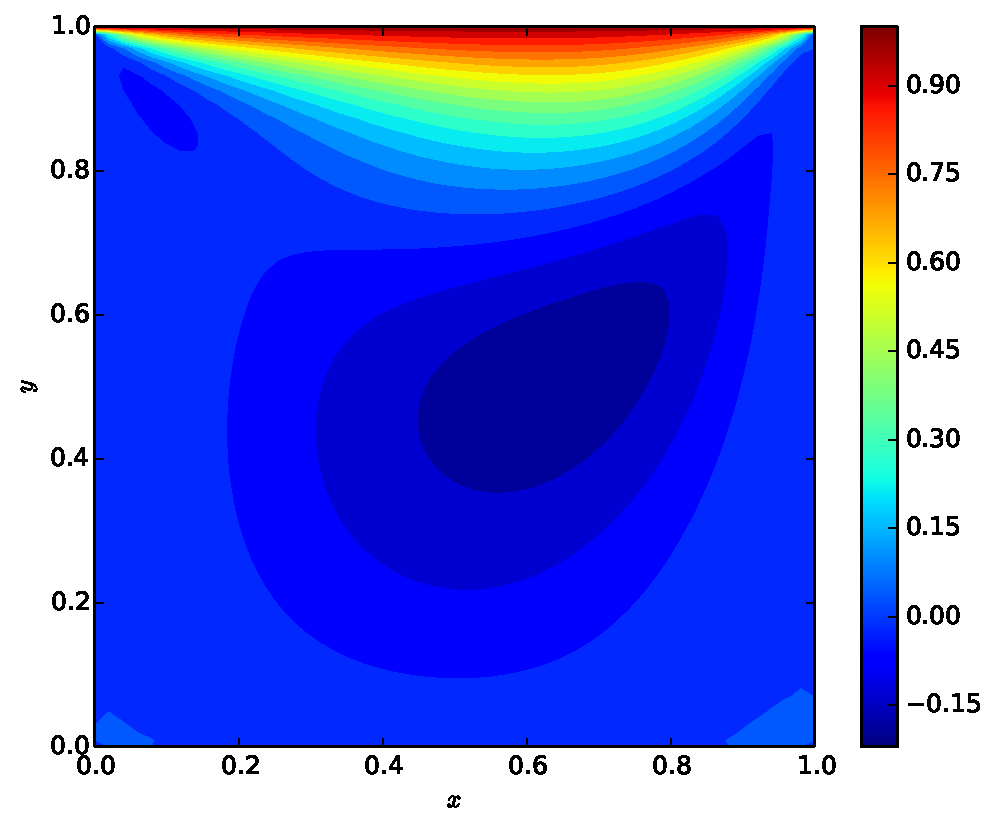
\includegraphics[width=0.4\linewidth]{../Cavity/u.pdf}
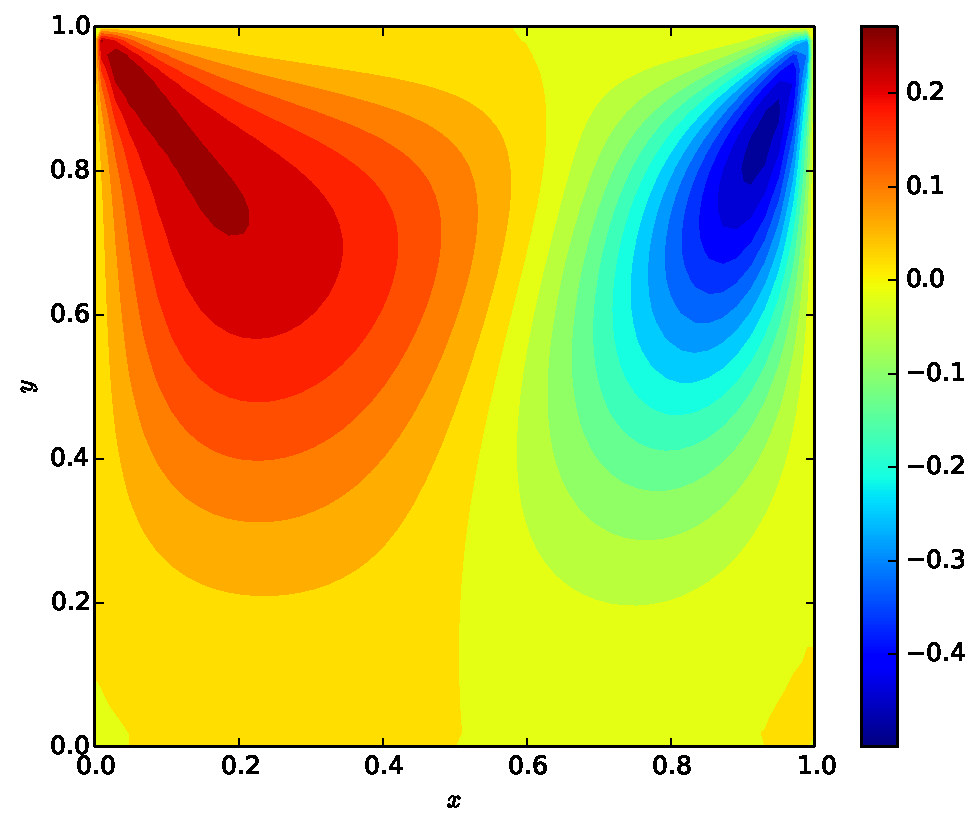
\includegraphics[width=0.4\linewidth]{../Cavity/v.pdf}

The below two plots show the vector plots of velocity magnitude (left) and the pressure contour (right).

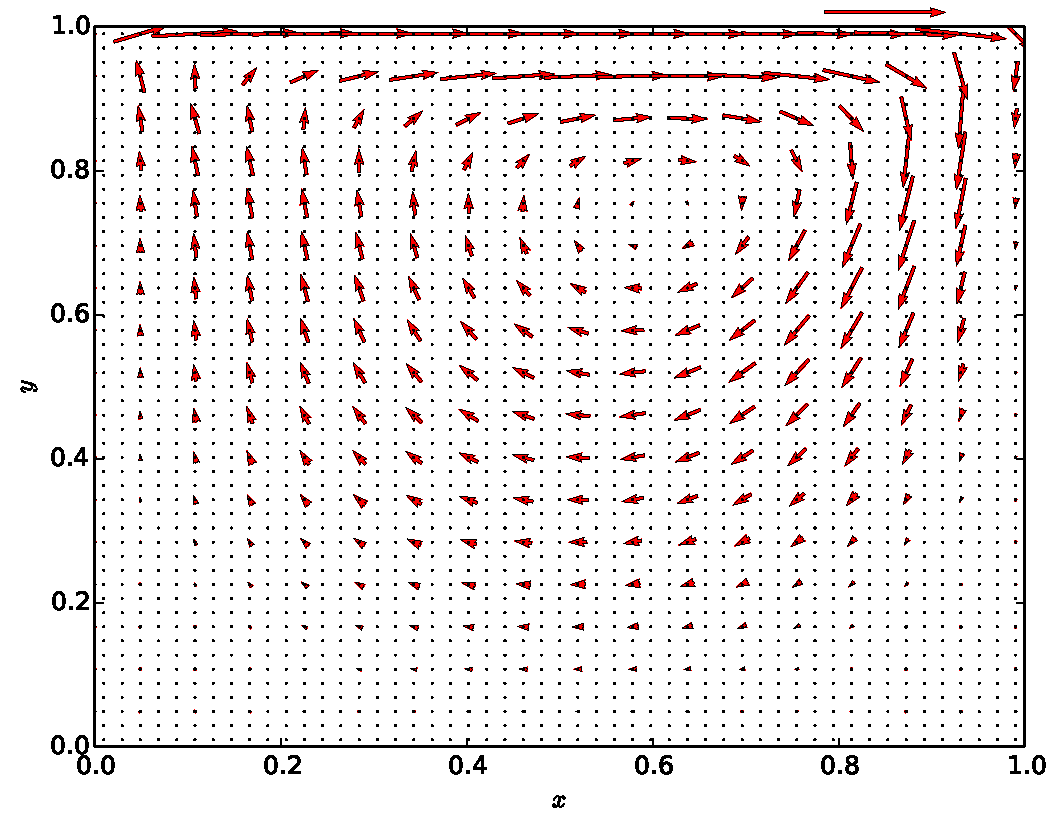
\includegraphics[width=0.4\linewidth]{../Cavity/uv.pdf}
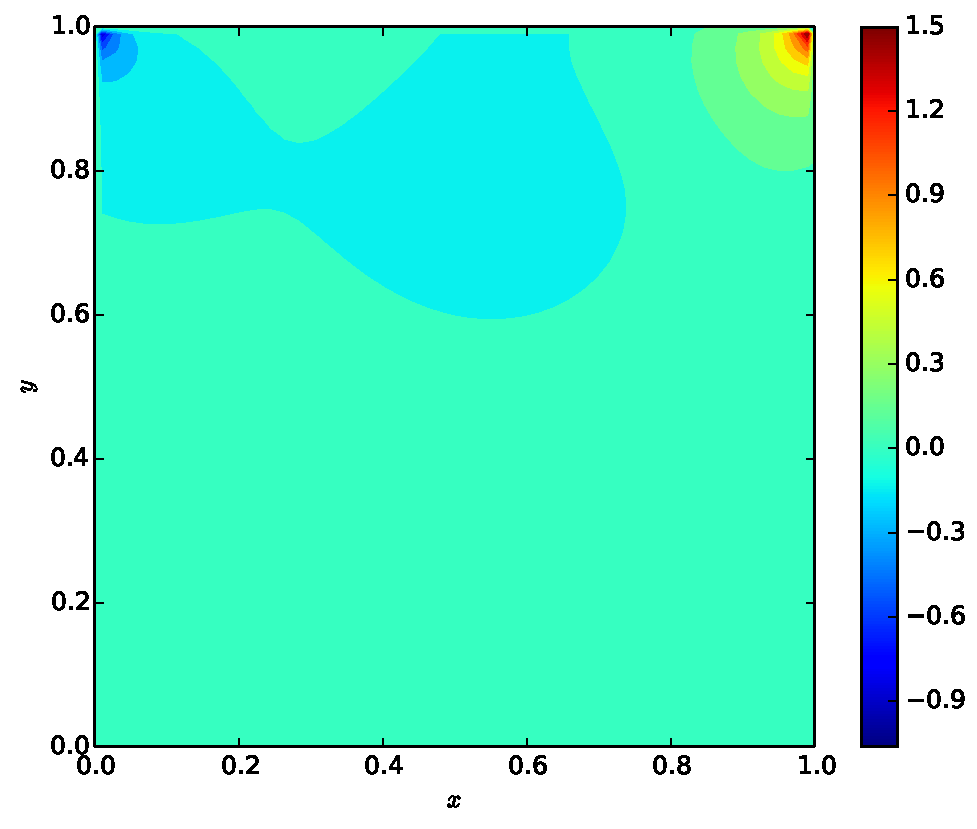
\includegraphics[width=0.4\linewidth]{../Cavity/p.pdf}

The below two plots show the error vs iterations (left) and the $x=0.5~u$ values (right).  

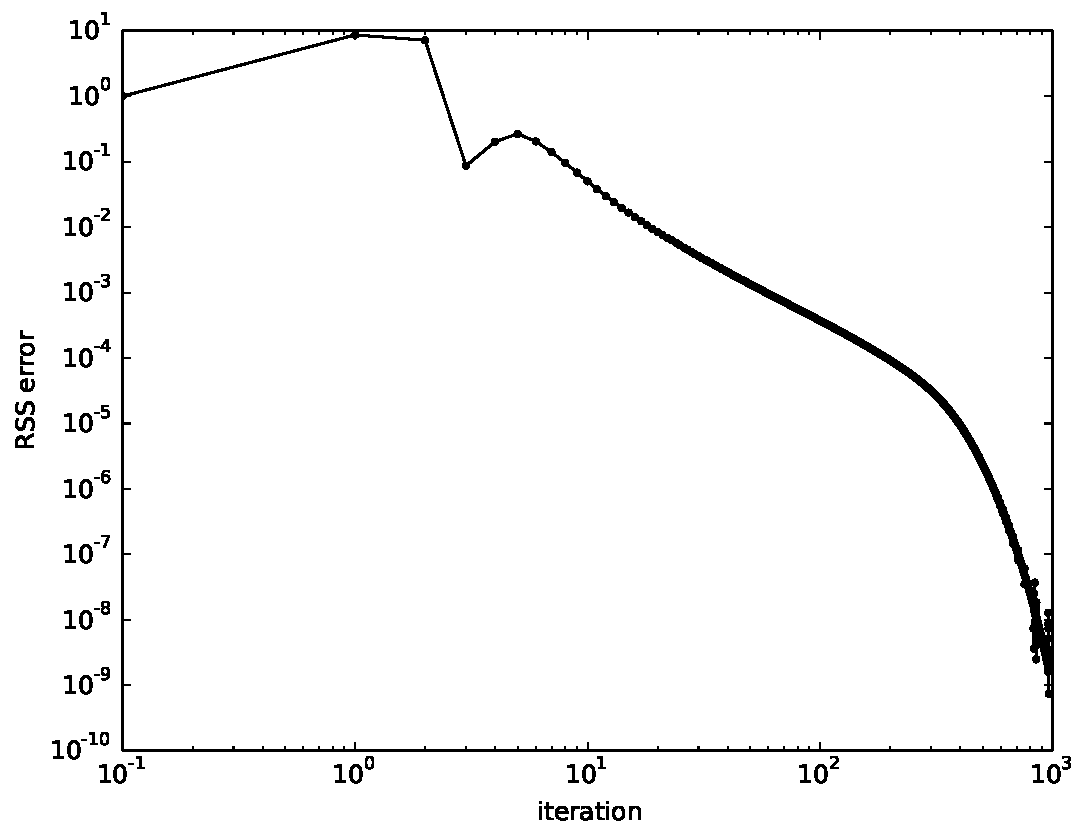
\includegraphics[width=0.4\linewidth]{../Cavity/iter.pdf}
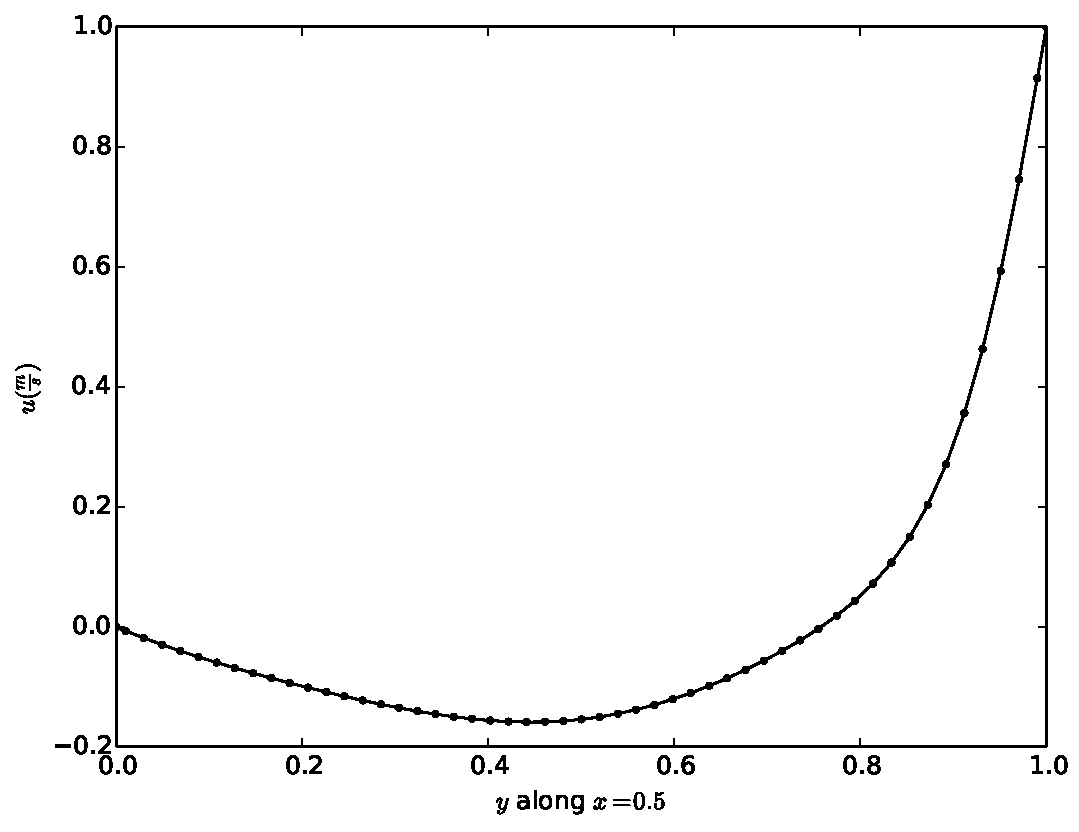
\includegraphics[width=0.4\linewidth]{../Cavity/u_spot.pdf}

The final mass imbalance for this 51X51 cell simulation was shown to be 1.60E-017.

\subsection{Channel Flow}

For this solution to function properly, the proper boundary condition needed to be applied.  Since the channel was long enough, the boundary condition to be applied was in the $u$ momentum solver.  We just set the outside condition to be equal to the flow directly upstream.  This allowed for flow to flow outside of the wall boundary.  

In addition to the plot provided in the above section.  The $u$ velocity for the centerline of the duct is shown.  The wall shear stress is also shown along both the upper and lower walls from the inlet to the outlet.  

The below two plots show the $u$ (left) and $v$ (right) velocity contours.

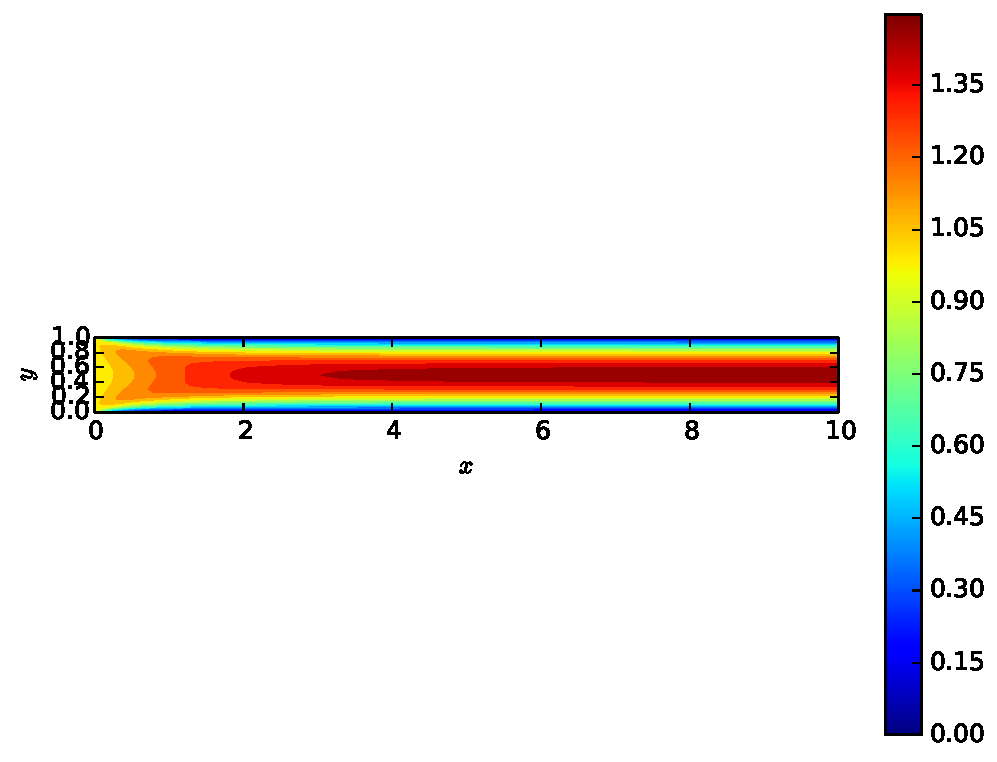
\includegraphics[width=0.4\linewidth]{../Channel/u.pdf}
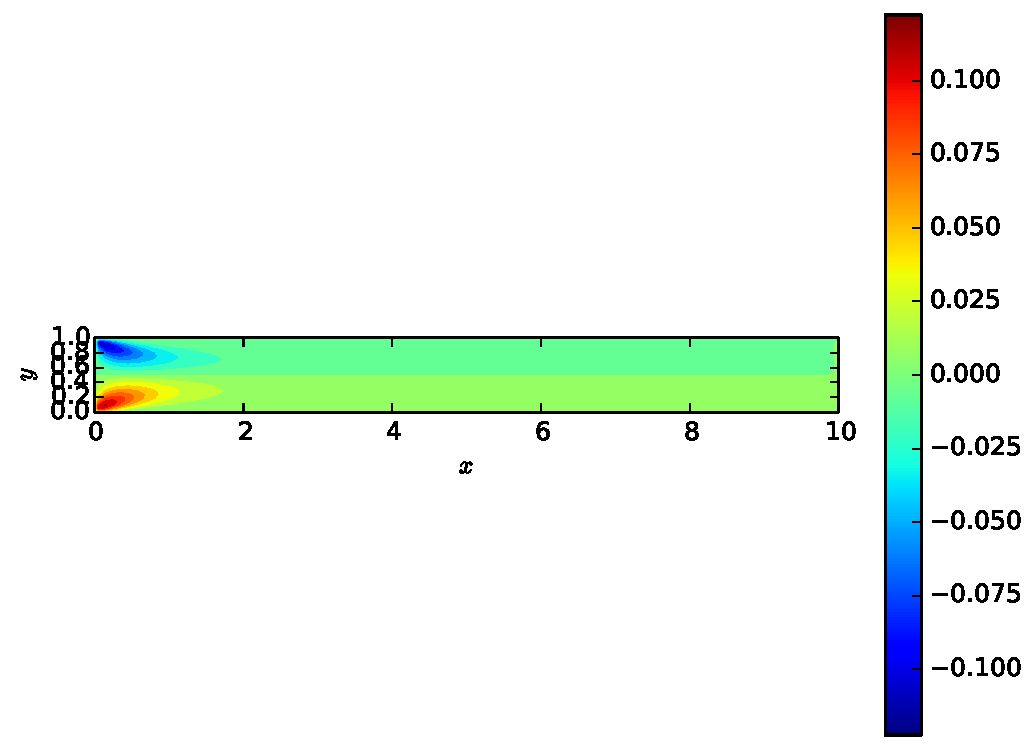
\includegraphics[width=0.4\linewidth]{../Channel/v.pdf}

The below two plots show the error vs iterations (left) and the $y=0.5~u$ values (right).  

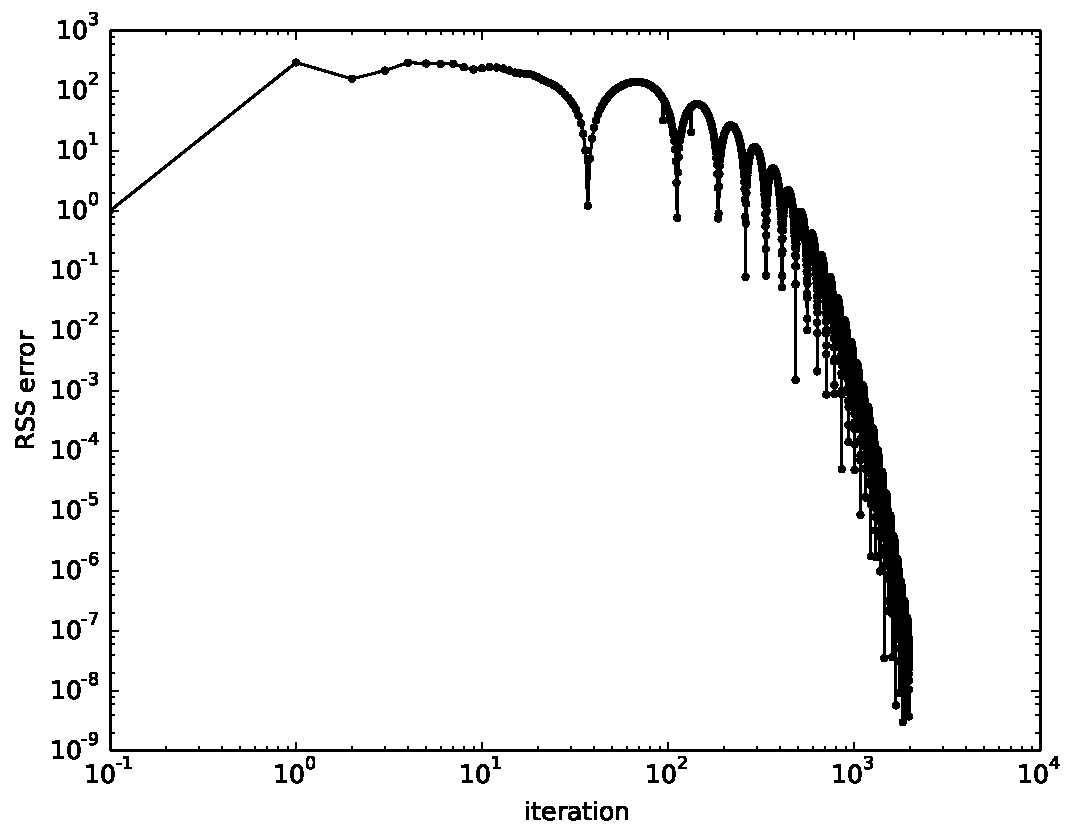
\includegraphics[width=0.4\linewidth]{../Channel/iter.pdf}
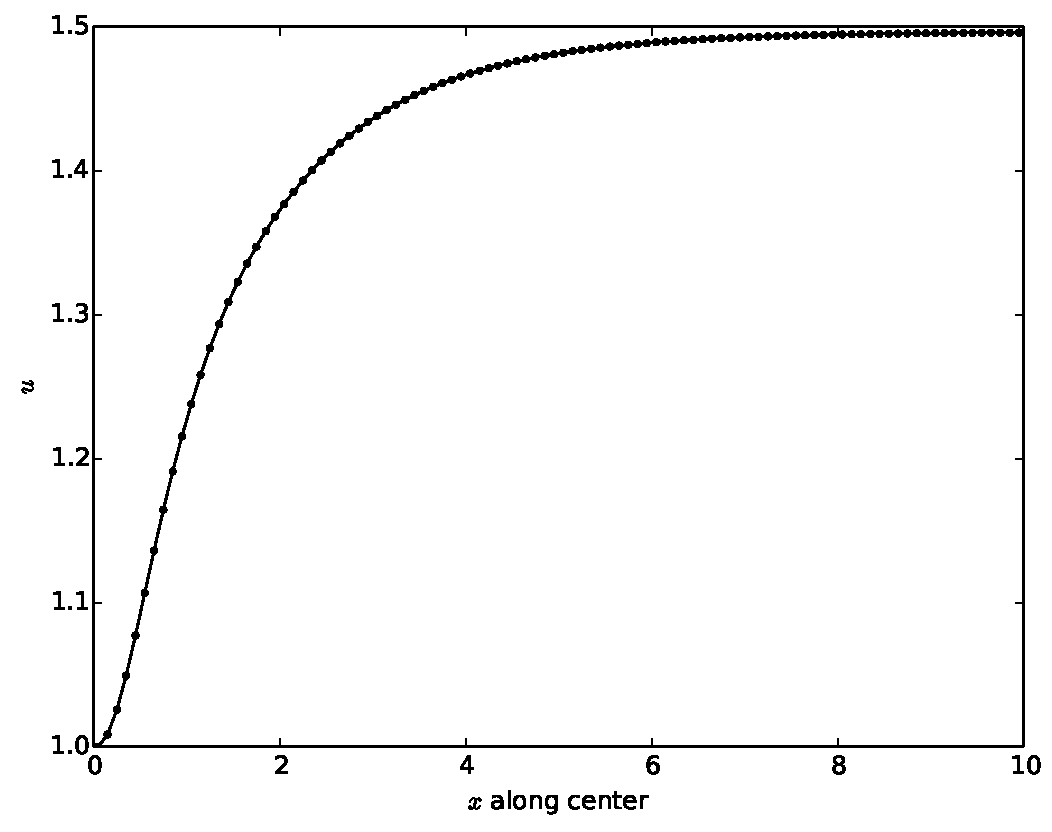
\includegraphics[width=0.4\linewidth]{../Channel/u_center.pdf}

The below two plots show the wall shear stress on the lower (left) and upper (right) surfaces.

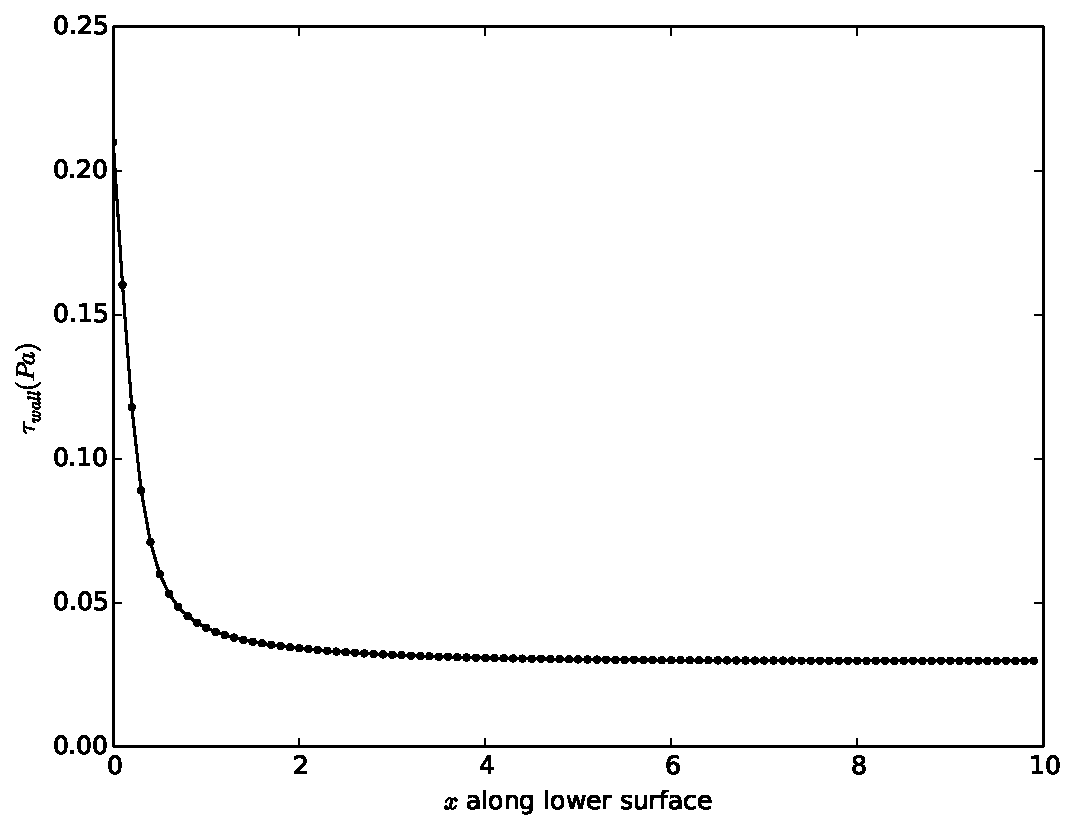
\includegraphics[width=0.4\linewidth]{../Channel/tau_lower.pdf}
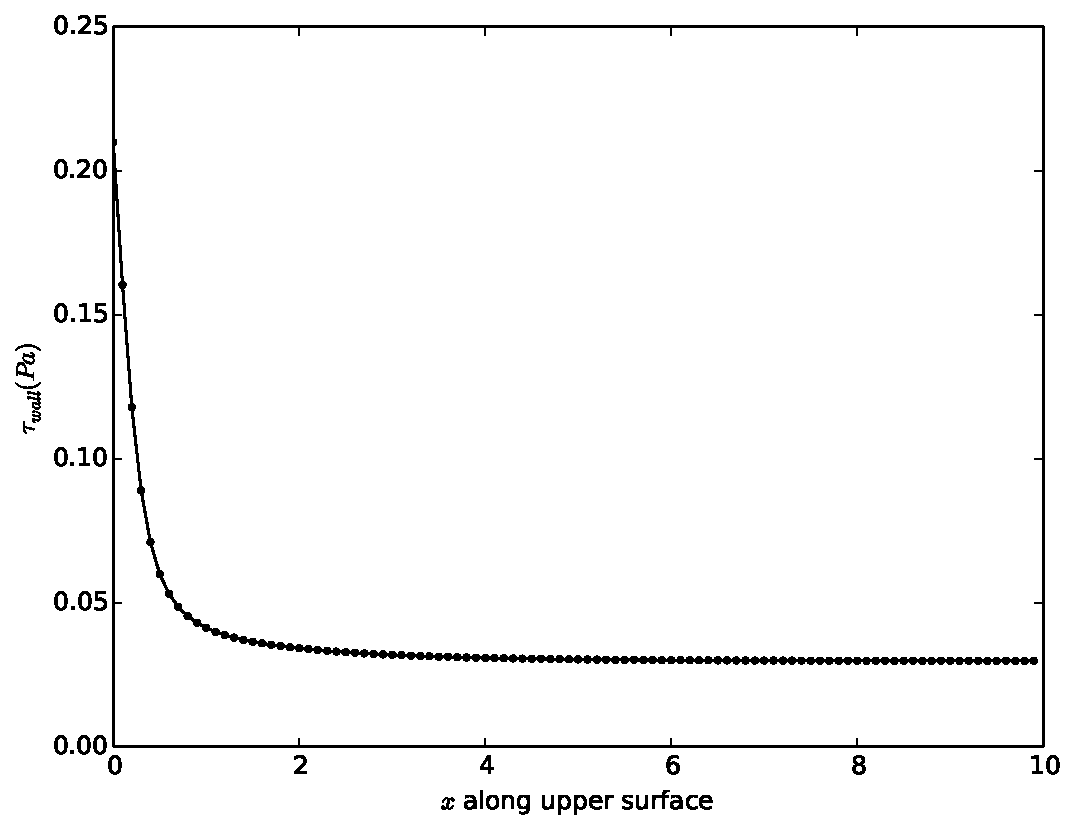
\includegraphics[width=0.4\linewidth]{../Channel/tau_upper.pdf}

The final mass imbalance for this 21X100 cell problem was shown to be 7.44E-023




%%%%%%%%%%%%%%%%%%%%%%%%%%%%%%%%%%%%%%%%%%%%%%%%%%%%%%%%%%%%%%%%%%%%%%

\section{CONCLUSION}

We have demonstrated a computational fluid dynamics solver for a driven cavity and for a channel flow study.  We have shown the staggered grid approach using two dimensional $u,v,$ and $P$ solvers.

%%%%%%%%%%%%%%%%%%%%%%%%%%%%%%%%%%%%%%%%%%%%%%%%%%%%%%%%%%%%%%%%%%%%%%

%\bibliographystyle{asmems4}
%\bibliography{asme2e}

%%%%%%%%%%%%%%%%%%%%%%%%%%%%%%%%%%%%%%%%%%%%%%%%%%%%%%%%%%%%%%%%%%%%%%

%\section*{FIGURES}



%%%%%%%%%%%%%%%%%%%%%%%%%%%%%%%%%%%%%%%%%%%%%%%%%%%%%%%%%%%%%%%%%%%%%%

\appendix

\section{Code}
\label{sec:code}

\subsection{Subroutines}
\lstinputlisting[language=Fortran]{../Project3_code/Types.f90}
\subsection{Main program}
\lstinputlisting[language=Fortran]{../Project3_code/Project3.f90}



\end{document}
